Virtualization is a way to emulate hardware in order to allow multiple operating systems to run concurrently on a physical system.  The hypervisor provides an abstraction and isolation of each guest to ensure protection. Virtualization allows data centers to reduce cost and power by overcommitting and sharing system resources across disparate operating systems with common hardware  (Figure \ref{virtStack}).

\begin{figure}[!h]
  \begin{center}
  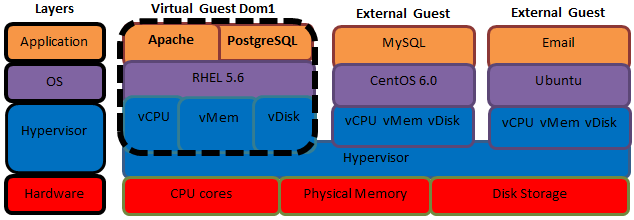
\includegraphics[width=6in]{images/LayersAll.png}
  \caption{\textbf{Virtualization Example}  Domain 1 is running with some external systems.  The hypervisor  divides, shares, and overcommits the physical resources between the 3 guest domains.  Each guest has access to virtual resources and not physical hardware.}
  \label{virtStack}
  \end{center}
\end{figure}

In a single server environment or HPC cluster there can be \emph{interference} \cite{paul} or \emph{system noise}\cite{tsafrir} caused by complex software layers (Application, OS, and Hardware), that causes poor application performance.  
The hypervisor, as well as multiple external guest virtual machines, compete for system resources and add to this interference.  Current performance tools in the virtual guests are unable to distinguish between performance problems in the guest machine and external interference.  We have developed a method to aggregate resource counters from multiple layers of virtualization to accurately diagnose interference as the root cause of a performance bottleneck. 

% Section 1.1
\subsection{Motivating Example}
A large US corportation, with over 10,000 employees and 200 franchises had a custom application for a retail business that sold and serviced merchandise.  A suite of applications which had been specifically written for this business consisted of a core inventory, service, accounting, and several other add-on services.  The OS consisted of Redhat based Linux with 2.6.18 kernel, Postgresql 8.3.6, and Apache 2.2.3 The hardware had 40 CPU cores (4 sockets 10 cores each) and 256 GB of RAM with a high end RAID SAN used for the data store.  At most times during the business day the system would run with less than 60\% total CPU and would cache nearly all data inside active RAM.   The system ran optimally for several months in this configuration, and was hosted in a data center.

\indent At some point the customer and data center decided to virtualize the application to add disaster recover and save power.  After several weeks the end users started to complain and enter trouble tickets about slow response times in the web server.  Application developers and support quickly found issues and developed fixes.   Usually these fixes were to reduce the number or reads or writes to some file in the filesystem.  However, after each fix, sometimes days later, a new problem would show up.  Eventually the database engineers and system engineers began examining the recurring problems.

\indent The symptom was that sometimes the system would go into a state where all 32 cores would go to 100\% CPU time, multiple threads would go to a “D state” \footnote{A procees in the D state is neither running nor sleeping.  It is "Uninterruptable sleep (usually IO)"} , and multiple processess would just not complete.   The additional CPU time was shown to be in \emph{System Time} and multiple tools confirmed this.  Memory and IO used on the guest and host server were consistent, and engineers monitoring the SAN did not see any latencies or problems measuring disk IO.  Sometimes this would only last a few seconds and sometimes it would last for hours. At some points the \emph{strace} output of Apache process would hang for several seconds on system calls to \emph{open}, \emph{lseek}, and \emph{write}.  See Figure \ref{fig:syscalls} for details.

\begin{figure}
%\begin{Verbatim}[frame=single]
\begin{Verbatim}
12:46:02 open("…", O_WRONLY|O_CREAT|O_
12:46:16 fstat64(61, {st_mode=S_IFREG| 
12:46:16 lseek(61, 0, SEEK_CUR) = 0 
12:46:24 write(61, "O:6_"..., 8192) =  
12:46:24 write(61, "R1339 "..., 8192)  
12:46:24 write(61, "ct "..., 8192) = 8 
12:46:31 write(61, "cription "..., 819  
12:46:31 write(61, ";s:11 "..., 8192)  
12:46:31 write(61, "7:for "..., 3288)  
12:46:31 close(61) = 0
\end{Verbatim}
\label{fig:syscalls}
\caption{\emph{strace} shows system calls to open, lseek, and write take up to 14 seconds to complete}
\end{figure}

\indent Looking at statistics in the VMM showed exactly what was noticed on the guest.  High CPU usage, but from the point of view of the VMM, there was no difference between guest time and kernel time and appeared as though there was a misbehaving guest application or guest kernel.  However, no symptoms appeared until the application was virtualized.  The guest was unable to perform profiling with hardware coutners on this version of the hypervisor \cite{serebrin} to see if there was a kernel bug.  Was there a bug or misconfiguration in the application, guest OS, hypervisor, or hardware?  Or was there just too much overhead from virtualization during peak usage?


% Section 1.2
\subsection{Measurement Challenges}
On a physical server, we can assume the hardware speed is known.  For a CPU we can measure in hertz or Floating Point Operations per Second (FLOPS), and for a disk we can measure in I/O per second (IOPS) or latency.  When that system is virtualized, the availability of the virtual resources are dynamic.  The resource may (or may not) be available to the guest and the performance tools become nearly meaningless.  Without knowledge of the availability, it is difficult to diagnose or find a root cause from a guest application. There is almost no way to distinguish between a poor running application, OS kernel issue, or external interference.  From the Hypervisor view, there is no information about the guest applications or guest kernel functions, so there is no way to relate a problem to a guest application.  Furthermore, the entity managing the hypervisor layer is likely a completely different organization than the entity managing the virtual guest. 

Since each guest machine only uses a portion of the available resources at any given time, the total resources allocated to all guest VMs can exceed the total physical resources \cite{huber2, amit, buell1}.   This idea of overcommitting resources is the same as preemptive multitasking, where multiple processes share a single CPU; and OS virtual memory, where the total memory available to applications exceeds the physical memory capacity.  In order to maximize resources, IT data centers overcommit the resources, with the hope that multiple virtual guest machines do not need all resources concurrently.  Even when the CPU and memory are not overcommitted there is still shared cache and memory bus.  For network and disk I/O multiple guests usually share access to a single physical resource, which can cause interference when accessed concurrently.

Existing performance tools fall into three categories, but they are unable to accurately diagnose or find a root cause of performance problems of production guest systems.  First, profiling tools are available on limited platforms, and require significant guest kernel and hypervisor support and coordination.  Additionally, profiling is a great tool for identifying problems in test and development, but may not be available on production systems.  
Second, performance monitoring tools are readily available on most every operating system.  They are very valuable for physical hardware but they assume that the resources are constant.  The performance data used by the tools when external systems are causeing interference is indistinguishable from a change in the application workload.
Finally, hypervisor tools can show each guest and the physical resources, but they do not have access to the applications in the guest.  There is no way to relate a problem seen in the hypervisor to specific processes in the guest or the guest kernel. 

% Section 1.3
\subsection{The growing importance of virtualization}
Due to the cost savings and decreased physical administration overhead, data centers and businesses are changing from physical server to virtualized environments. In 2008 Gartners research found that virtualization is not just for server consolidation, but for ”efficient use of shared resources” \cite{gartners}.  They attribute the growth of cloud computing to standardization of technologies, increase use of the Internet, and virtualization.  Research from Ramya and Edwin show tremendous growth in Platform As A Service (PAAS) where an entire system platform is dynamically provisioned in a cloud computing service \cite{ramya}. The NIST explicitly states that for PAAS the consumer does not manage or control the underlying infrastructure including networks, servers, and storage. They state that cloud systems should provide a \emph{measured service} and resources utilization is ”monitored, controlled, and reported” by providing transparency of the service \cite{nist}.  Massive data centers are able to provide virtual systems, and manage large clusters of shared resources, for a fraction of the price of building a physical server for each customer.

\subsection{Contributions}
This research presents a method for analyzing performance data at runtime in the guests and Virtual Machine Monitor (VMM).   With this framework we can detect the I/O interference by sharing physical and virtual I/O performance statistics between multiple guests.  We believe that this method can be extended to find interference from other resources.  This could significantly reduce time spent troubleshooting and analyzing performance problems in virtualized environments.
\newline

The thesis statement is that we can measure external interference by relating virtual and physical resource usage across multiple layers.
\newline

\noindent
The contributions of this thesis are:
\begin{enumerate}
% \item \textbf{Layers} Define the layers of abstraction in virtual environments.
% \item \textbf{Resources} Define the physical and virtual resources which need to be measured.
% \item \textbf{Counters} Examine some common counters, and metrics which can measure resource utilization.
\item \textbf{Overhead} We Designed a new method to measure the overhead of virtualization.
\item \textbf{Interference} We Designed a method to collect resource metrics at several layers and quantify the I/O interference from virtualization.
\item \textbf{Test Suite} Developed an interference test suite that causes measurable I/O interference in a virtualized server.
\end{enumerate}

The remainder of this document is organized as follows:  In section 2 we examine related work.  In section 3 we define our methodology.  Section 4 shows our experimental results for two different architectures.   We conclude and discuss future work in section 5.

